\chapter{Integrated Results and Error Analysis}
\label{ch:results}

\section{Cross-experiment view}

Table~\ref{tab:cross-experiment} collects the principal and strongest observed
results without treating them as directly exchangeable. V1 and V2 use the
controlled 69-person cohort; V2 adds boundary guards. V3 and V4 use all 88
people and a different fold seed. V3 and V4 are the cleanest paired comparison
because they share the same input arrays and outer splits.

\begin{table}[htbp]
\centering
\small
\begin{tabularx}{\textwidth}{lXrr}
\toprule
\textbf{Stage} & \textbf{Reported procedure} & \textbf{Mean BA} & \textbf{Status}\\
\midrule
V1 & PCA/NMF rank 8 plus logistic regression & 54.1\% & Exploratory maximum\\
V2 & Complete inner-selected pipeline & 47.3\% & Primary endpoint\\
V2 & Tucker/HOSVD family & 56.0\% & Secondary family\\
V3 & Complete inner-selected pipeline & 52.0\% & Primary endpoint\\
V3 & Same-cohort spectral control & 55.8\% & Secondary family\\
V4 & Complete inner-selected pipeline & 54.5\% & Primary endpoint\\
V4 & Tuned RBF SVM family & 59.7\% & Secondary family\\
V4 & TT/spectral fusion family & 59.1\% & Secondary family\\
\bottomrule
\end{tabularx}
\caption{Cross-experiment results and their correct inferential status.}
\label{tab:cross-experiment}
\end{table}

\begin{figure}[htbp]
\centering
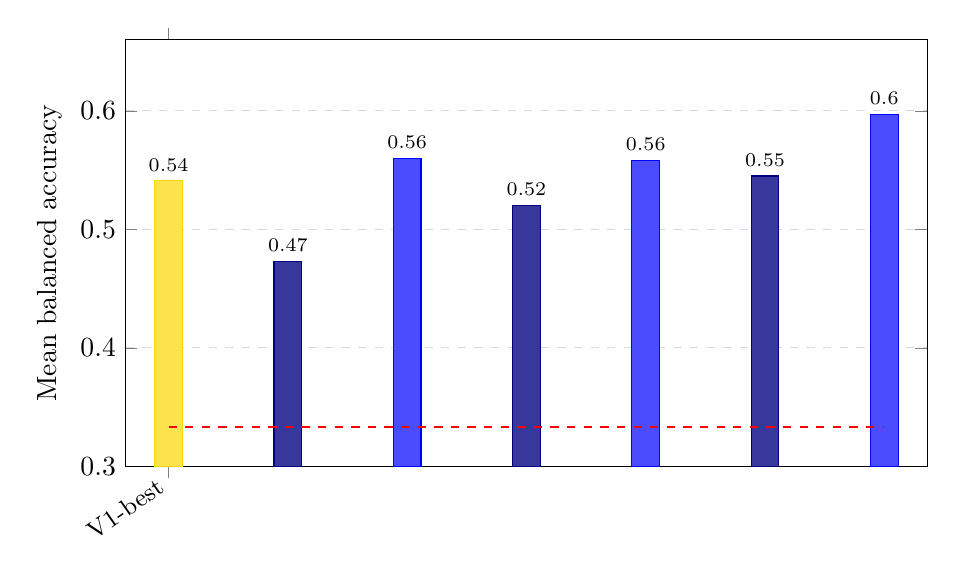
\begin{tikzpicture}
\begin{axis}[
  ybar,
  bar shift=0pt,
  width=0.97\textwidth,
  height=70mm,
  ymin=0.30,ymax=0.66,
  ylabel={Mean balanced accuracy},
  symbolic x coords={V1-best,V2-primary,V2-Tucker,V3-primary,V3-spectral,V4-primary,V4-SVM},
  xtick=data,
  x tick label style={rotate=35,anchor=east,font=\small},
  ymajorgrids=true,
  grid style={dashed,gray!30},
  nodes near coords,
  every node near coord/.append style={font=\scriptsize},
  enlarge x limits=0.06
]
\addplot[fill=Gold!70,draw=Gold] coordinates {(V1-best,0.541)};
\addplot[fill=Navy!78,draw=Navy] coordinates {(V2-primary,0.473) (V3-primary,0.520) (V4-primary,0.545)};
\addplot[fill=Blue!70,draw=Blue] coordinates {(V2-Tucker,0.560) (V3-spectral,0.558) (V4-SVM,0.597)};
\draw[dashed,thick,Red] (axis cs:V1-best,0.333) -- (axis cs:V4-SVM,0.333);
\end{axis}
\end{tikzpicture}
\caption{Experiment progression. Navy bars are predeclared complete-pipeline endpoints; blue bars are secondary best-family results; the V1 maximum is exploratory. The dashed baseline is 33.3\% balanced accuracy.}
\label{fig:experiment-evolution}
\end{figure}


The 59.7\% SVM value is the highest retained result, but it is not an accuracy
ceiling and cannot be promoted over the V4 primary endpoint. The project has no
untouched external test cohort. Repeated outer folds also share much of their
training data, so the repeat SD is descriptive rather than a confidence
interval.

\section{Metric definitions}

For confusion matrix $M$ with classes $g\in\{\AD,\FTD,\CN\}$, class recall is

\begin{equation}
R_g=\frac{M_{gg}}{\sum_j M_{gj}},
\end{equation}

and balanced accuracy is

\begin{equation}
\BA=\frac{1}{3}\sum_g R_g.
\end{equation}

Always predicting one class gives 33.3\% balanced accuracy. In the 88-person
cohort, always predicting \AD{} gives 40.9\% ordinary accuracy because \AD{} is
the largest class. Macro F1 gives each class equal weight after combining
precision and recall, making it useful alongside \BA{}.

\section{Diagnosis-specific error pattern}

\FTD{} is the consistent weakness. In the V1 PCA result, \FTD{} recall is
30.4\%. V2 Tucker improves it to 50.7\%, but V4 classifier-family values remain
30.4--43.5\%. The strongest V4 SVM family has mean recalls of 57.4\% \AD{},
43.5\% \FTD{}, and 78.2\% \CN{}. The model is therefore much better at
recognizing controls than at separating the two dementia groups.

This pattern is plausible for three non-exclusive reasons:

\begin{enumerate}
  \item \textbf{Independent sample limitation.} Only 23 \FTD{} people exist.
  Thousands of additional four-second windows stabilize each person's features
  but do not provide new independent anatomy or disease variability.
  \item \textbf{Phenotypic overlap.} Resting spectral slowing and covariance
  changes need not uniquely separate \AD{} from \FTD{} in a small heterogeneous
  routine-EEG cohort.
  \item \textbf{Representation mismatch.} The strongest features may emphasize
  healthy-versus-dementia differences, while the finer AD-versus-FTD distinction
  may require connectivity, topography, longer temporal structure, or external
  clinical information not used here.
\end{enumerate}

\section{What tensorization contributed}

The results support a nuanced conclusion:

\begin{itemize}
  \item Tensorization is useful for imposing explicit channel-frequency-time or
  channel-lag structure and for testing low-rank hypotheses.
  \item Tucker/HOSVD is the strongest corrected V2 family at 56.0\%, showing that
  multilinear compression can be competitive.
  \item V3 spectral controls outperform every waveform-only branch, so a more
  ``raw'' representation is not automatically better.
  \item V4 fusion reaches 59.1\%, but its feature selector can choose spectral
  dimensions; the experiment does not prove an isolated TT gain.
  \item Waveform TT has high instability in V4 (11.7 pp repeat SD), suggesting
  sensitivity to the available training people and selected classifier.
\end{itemize}

The correct claim is that structured tensor methods were implemented, tested,
and compared under leakage-aware validation. The data do not support a claim
that tensor decomposition consistently dominates spectral baselines.

\section{Classifier effects}

V4 shows that classifier choice matters within the existing representations.
RBF SVM is strongest at 59.7\%, with a small descriptive repeat SD. Random forest
and XGBoost follow at 58.3\% and 57.6\%. The nonlinear kernel appears better
matched to the selected low-dimensional feature geometry than the tested boosted
trees. XGBoost remains useful because it rules out the assumption that a modern
tree ensemble must be best on this small participant-level table.

The automatic pipeline selects SVM in 7 outer fits, logistic regression in 5,
and random forest, XGBoost, and supervised TT once each. It selects fusion in 7
folds, spectral features in 7, and supervised TT once. This heterogeneity
explains why a single globally attractive family may still differ from the
complete fold-wise primary endpoint.

\section{Optimization effects}

V3's supervised TT reaches its 100-iteration cap in every original fit. Raising
the cap to 2,000 does not improve the fixed-model mean. V4 instead changes the
objective by strengthening the core anchor and reducing ranks, leading to
200/285 reported convergences. Predictive performance remains only 50.9\% for
the supervised TT family. Therefore:

\begin{quote}
Better numerical convergence is neither sufficient nor synonymous with better
generalization. Optimization quality, model bias, and data information content
must be evaluated separately.
\end{quote}

\section{Was more data needed?}

Using leftovers is worthwhile because it adds 19 people and 4,828 valid leftover
windows to the full-cohort analysis. Yet the main shortage remains independent
\FTD{} participants. Future data collection should prioritize new \FTD{} people
from an external site, plus an untouched validation cohort. Extra windows from
the same 23 people have diminishing value after per-person features stabilize.

The existing learning curve is too small and noisy to specify a required sample
size. A defensible sample-size study would use learning curves repeated over
many participant subsamples, preserve the three-class endpoint, and quantify
uncertainty. Until then, a statement such as ``we need exactly 50 more people''
would be invented rather than evidence-based.

\section{Fairness and confounding checks}

The controlled cohort broadly matches age, sex, duration buckets, people, and
window counts while retaining natural variation. The full cohort uses all
available people and corrects only loss weighting. Neither design uses protected
or clinical metadata as predictors. Nevertheless, the dataset is a single-site
clinical cohort and subgroup performance by age/sex has not been externally
validated. Demographic audit reduces obvious confounding; it does not establish
fairness or generalizability.

